
\section{Static Compilation}
\label{sec:compiler}

Once a \peft model is registered, \sys compiles it into a parallel computation graph (PCG)~\cite{unger2022unity}. To optimize finetuning performance, \sys applies two key static compilation optimizations to discover an optimized PCG: {\em dependent parallelization} (\S\ref{subsec:parallelization}) and {\em graph pruning} (\S\ref{subsec:pruning}).
%

\subsection{Dependent Parallelization}
\label{subsec:parallelization}

To minimize memory overhead, \sys allows finetuning and inference tasks to utilize the same backbone LLM and share memory allocated for both model weights and intermediate activations. This approach avoids redundant memory consumption while requiring the parallelization strategies of the \peft models to be compatible with that of the backbone LLM, a task termed {\em dependent parallelization}.

Existing auto-parallelization approaches like Alpa~\cite{zheng22-alpa} and Unity~\cite{unger2022unity} can identify optimal parallelization strategies for backbone LLMs.
\Sys extends the optimization target to also include the bypass networks in \peft models.
To achieve this goal, \sys generalizes the {\em parallel computation graph} (PCG) abstraction introduced in Unity~\cite{unger2022unity} by associating a {\em state} field with tensor dimension.

\Cref{fig:pcg_states} shows the four possible tensor states when parallelizing a tensor, including {\em non-parallel} ({\tt -}), {\em partitioned} ({\tt |}), {\em replicated} ({\tt =}), and {\em pre-reduce} ({\tt +}), as well as the state transitions.
Given the fixed parallelization of the backbone LLM, \sys searches for an optimal PCG for each bypass network by enumerating possible parallelization operators---{\tt partition}, {\tt combine}, {\tt replicate}, and {\tt reduce}---inferring output tensor states, and validating their compatibility.
\Cref{fig:candidate_pcg} shows four candidate PCGs discovered by \sys for parallelizing a LoRA network. To select the best strategy, \sys reuses Unity's profiling-based cost model~\cite{unger2022unity} and chooses the candidate PCG with the lowest estimated execution cost.


\begin{algorithm}[t]
\caption{Static graph pruning. For an operator $n$, $\textproc{UpdateInput}(n, \m{O}(n))$ returns a set of input tensors needed in order only to compute $\m{O}(n)$ of the operator.}
\label{alg:graph_pruning}
\begin{algorithmic}[1]
\State {\bf Inputs:} PCG of a PEFT model $\m{G}$
\State {\bf Outputs:} $\m{A}$ is a set of tensors to be memorized, $\m{R}$ is a set of tensors to be rematerialized
% \State \Comment{Step 1: computation graph pruning}
\LeftComment{Step 1: computation graph pruning}
\State $\overline{\m{G}} = \Call{ReverseAutoDiff}{\m{G}}$
\State $\m{Q} = \emptyset$ \Comment{$\m{Q}$ is a queue of updated operators}
\For{operator $n \in \overline{\m{G}}$}
%\State $\m{O}(n) = \m{O}(n) \setminus \m{B}$ \Comment{$\m{B}$ is the set of gradients to the backbone LLM}
\For{output tensor $t \in \m{O}(n)$}
\If{$t$ is the weight gradient of the base LLM}
\State $\m{O}(n) = \m{O}(n) \setminus \{t\}$
\State $\m{I}(n) = \Call{UpdateInput}{n, \m{O}(n)}$
\State $\m{Q}$.push\_back($n$)
\EndIf
\EndFor
\EndFor
\While{$\m{Q}$ is not empty}
\State $n = \m{Q}$.pop\_front()
\For{output tensor $t \in \m{O}(n)$}
\If{$\nexists u. t \in \m{I}(u)$ }
\State $\m{O}(n) = \m{O}(n) \setminus \{t\}$
\State $\m{I}(n) = \Call{UpdateInput}{n, \m{O}(n)}$
\State $\m{Q}$.push\_back($n$)
\EndIf
\EndFor
\EndWhile
\State $\m{A} = \emptyset$
\For{operator $n \in \m{G}$}
\For{tensor $t \ in \m{O}(n)$}
\If{$\exists u \in \overline{\m{G}}. t \in \m{I}(u)$}
\State $\m{A} = \m{A} \cup \{ t\}$
\EndIf
\EndFor
\EndFor
% \Statex \Comment{Step 2: opportunistically rematerializing tensors}
\LeftComment{Step 2: opportunistically rematerializing tensors}
\For{tensor $t \in \m{A}$}
\State Let $n$ be the operator that outputs $t$ (i.e., $t \in \m{O}(n)$)
\If{$\m{I}(n) \subseteq \m{A}$ and $\Call{Cost}{n} < threshold$}
\State $\m{A} = \m{A} \setminus \{t\}$, $\m{R} = \m{R} \cup \{t\}$
\EndIf
\EndFor
%\State \Comment{Step 3: tensor compression}
\State {\bf return} $\m{A}, \m{R}$
%\Function{aaa}{}
%\EndFunction
\end{algorithmic}
\end{algorithm}

\begin{figure}[t]
    \centering
    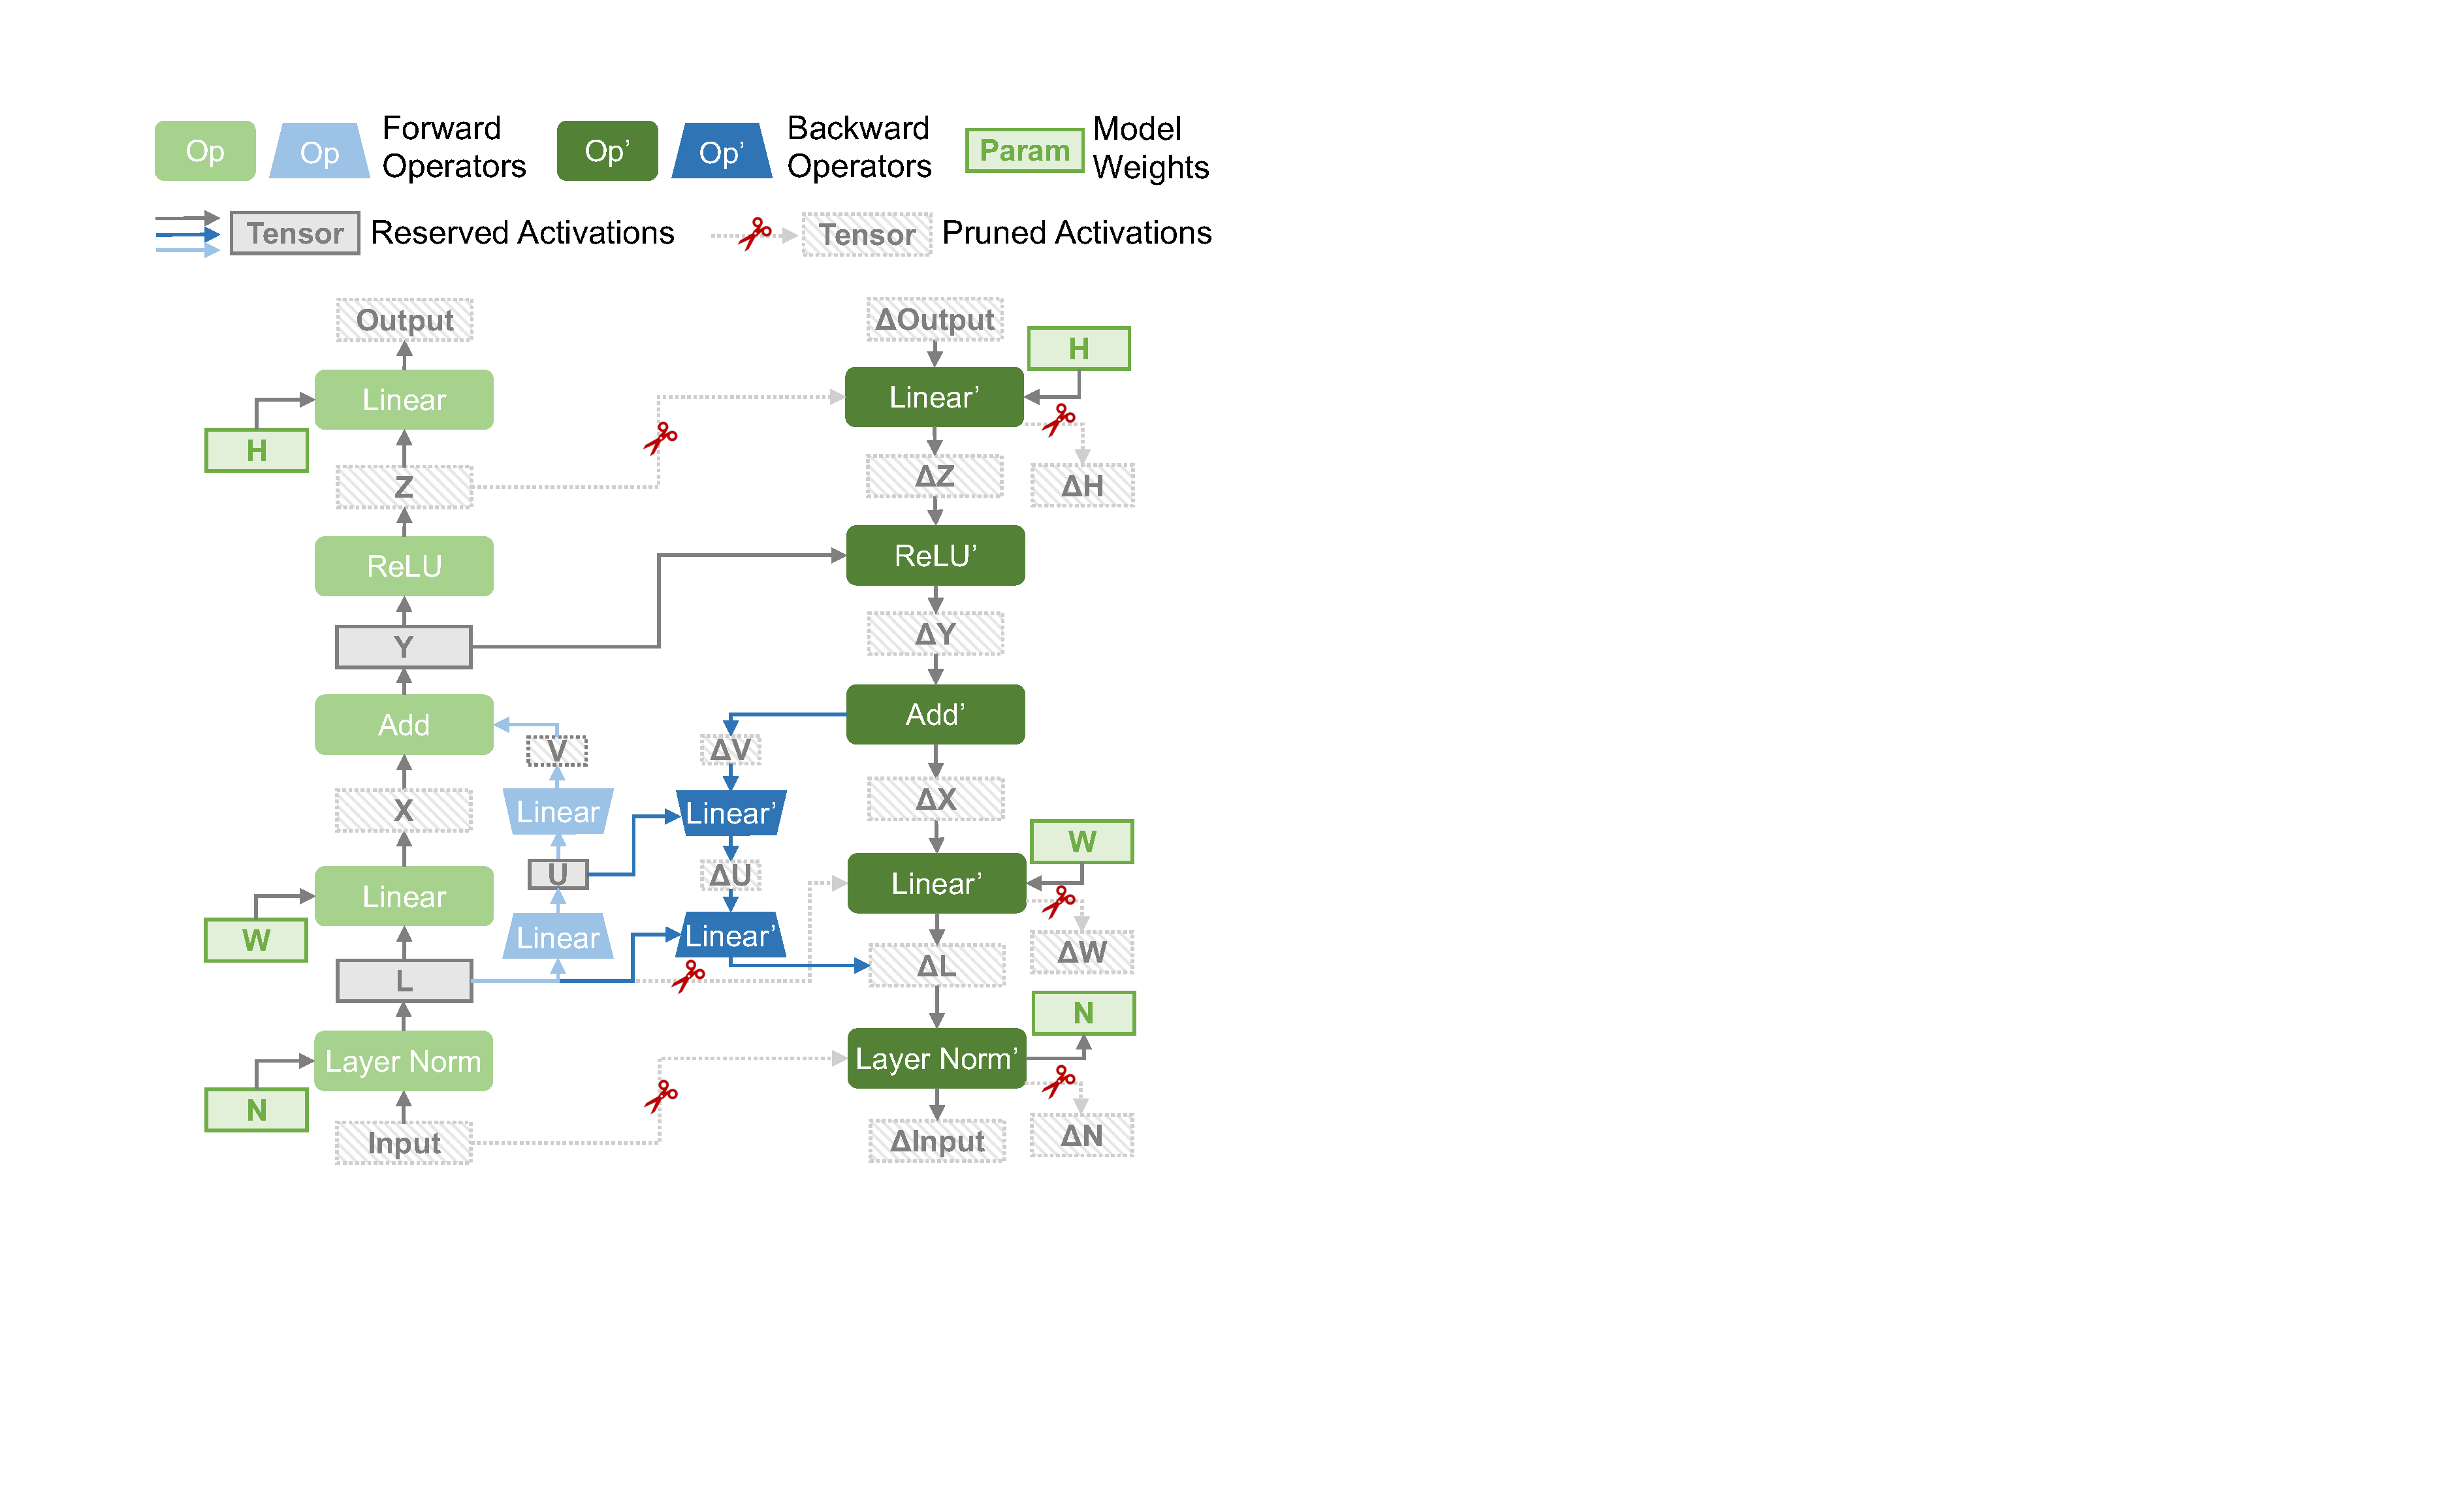
\includegraphics[width=0.8\linewidth]{figs/graph_pruning2.pdf}
    \caption{Static graph pruning for an MLP model with LoRA.}
    \label{fig:graph_pruning}
\end{figure}


\begin{figure*}[t]
    \centering
    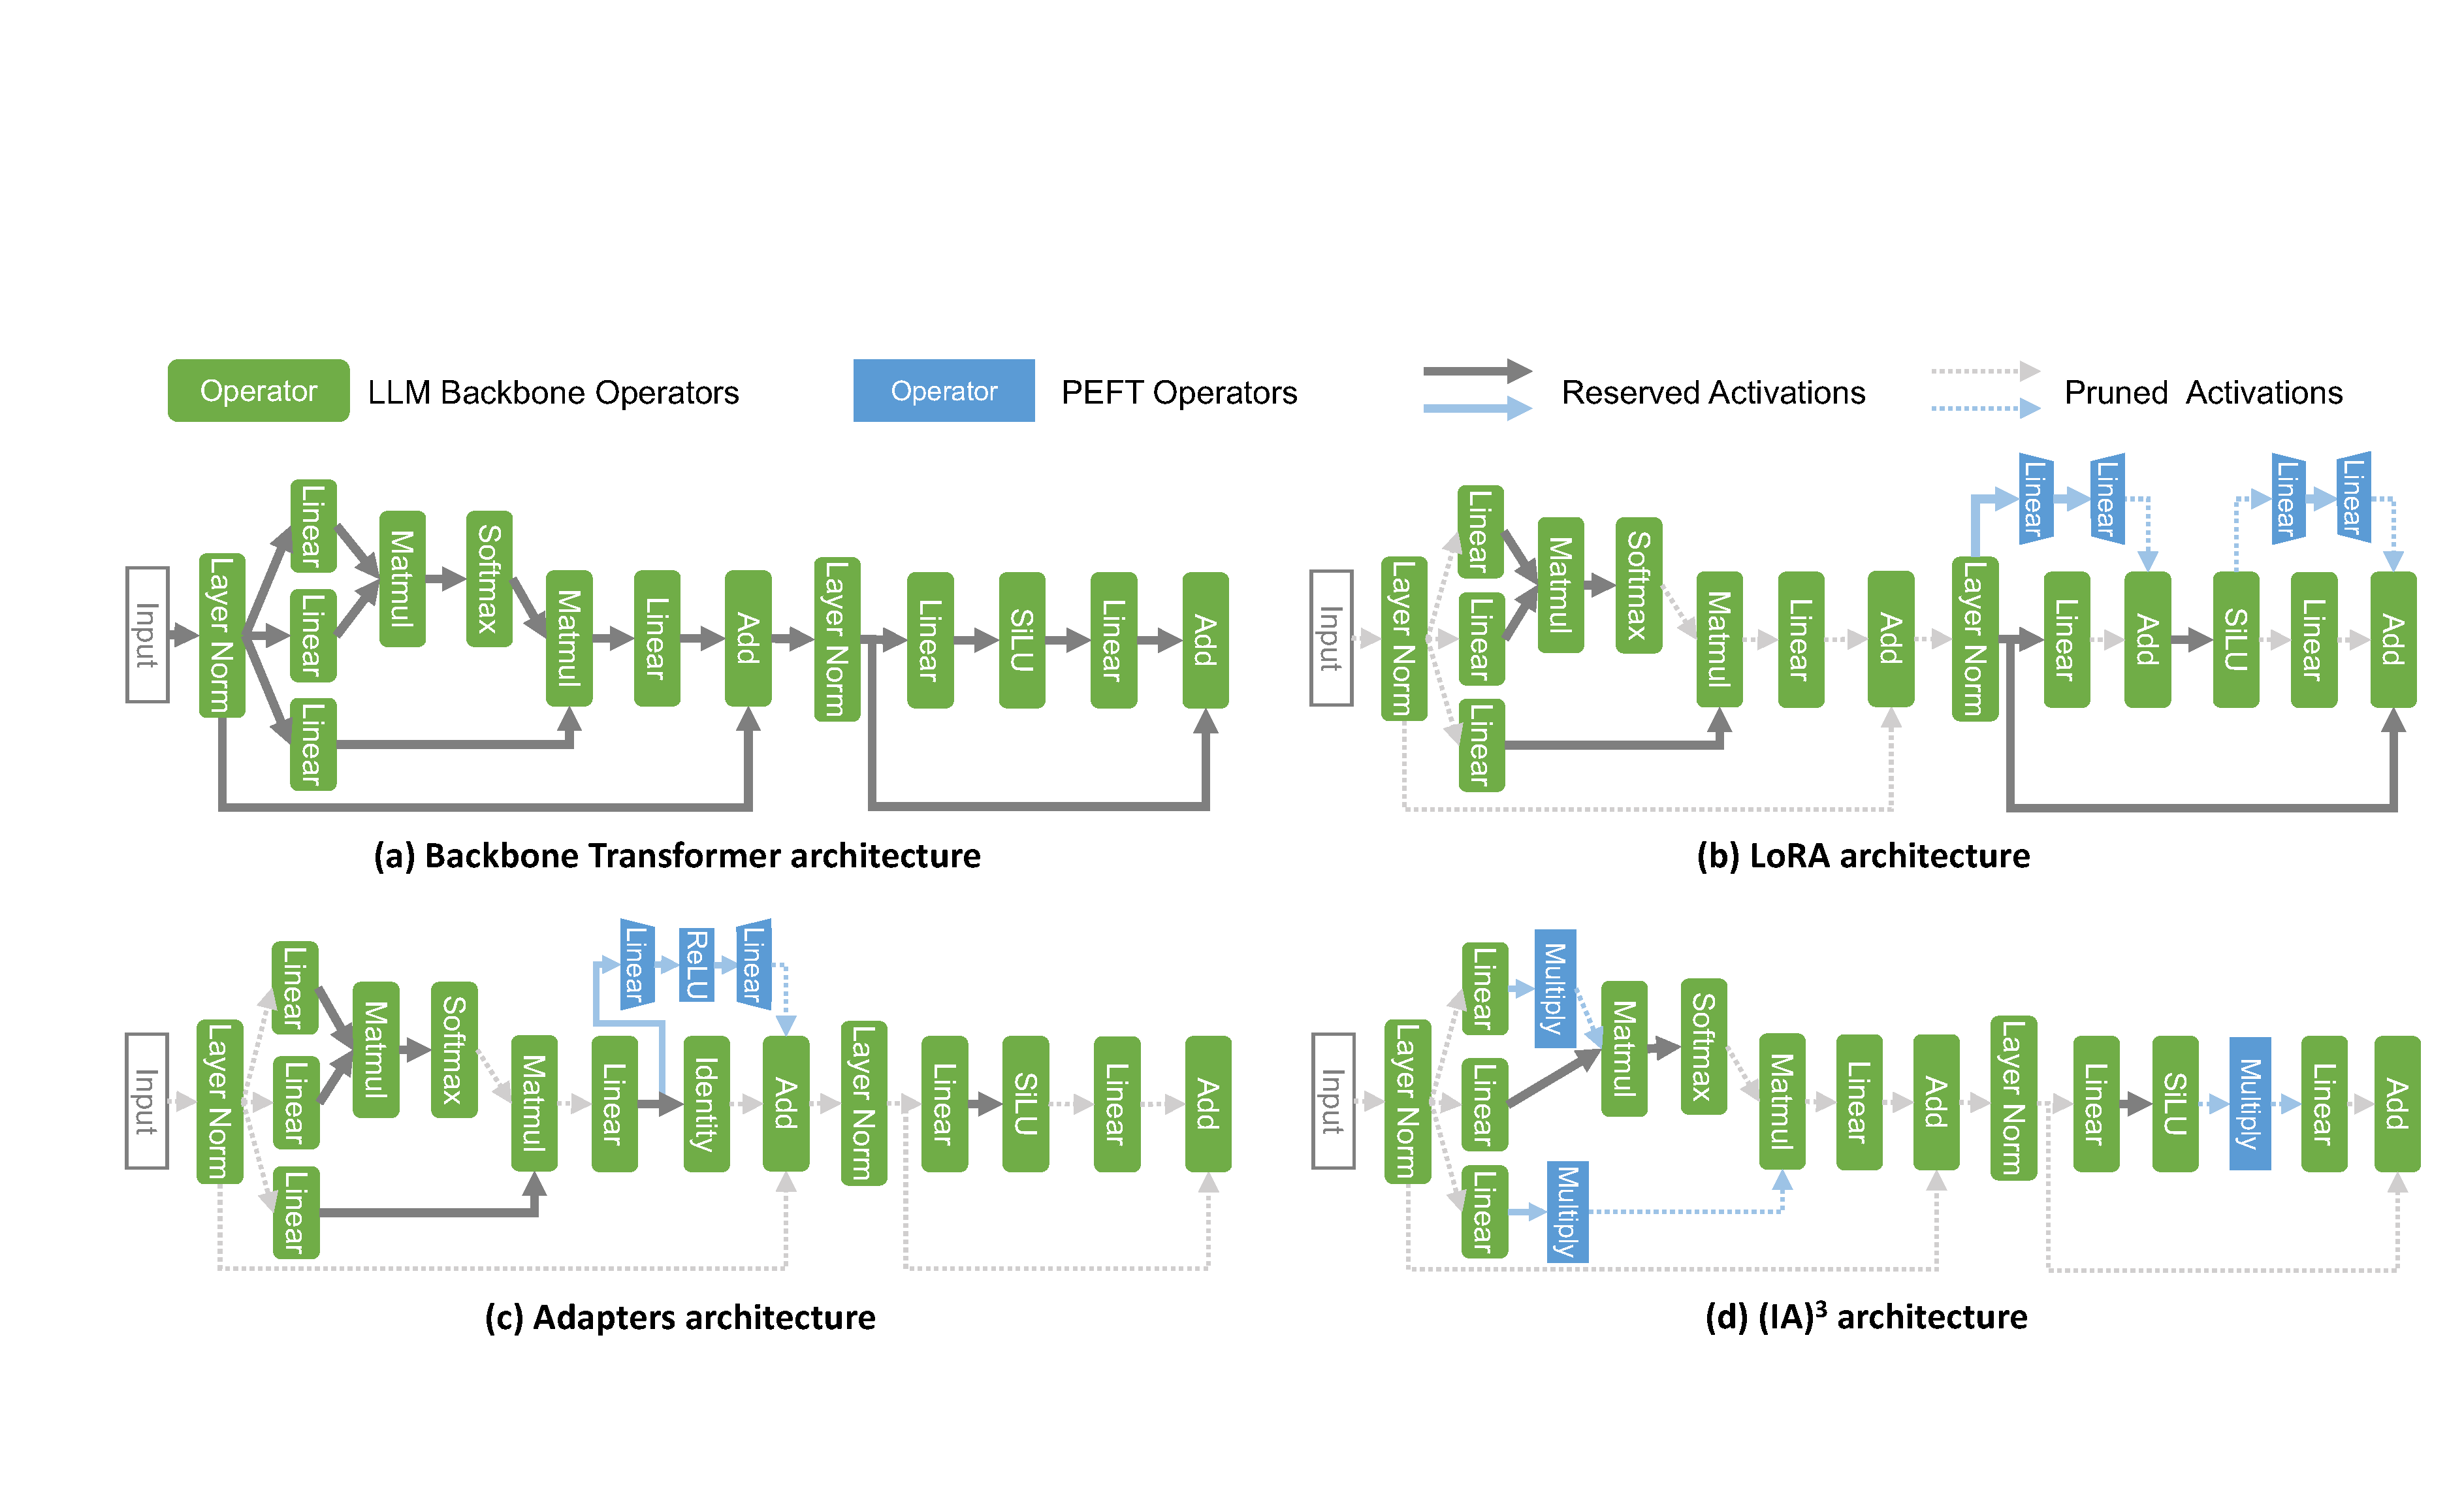
\includegraphics[width=0.85\textwidth]{figs/architecture2.pdf}
    \caption{An overview of existing parameter-efficient finetuning (PEFT) methods. Green boxes show the operators of the backbone LLM, while blue boxes are the operators introduced by different PEFT methods. Arrows represent intermediate activations to be reserved and the dashed arrows demonstrate they are pruned by \sys.}
    \label{fig:peft-methods}
\end{figure*}

\subsection{Graph Pruning}
\label{subsec:pruning}

\begin{figure*}[t]
    \centering
    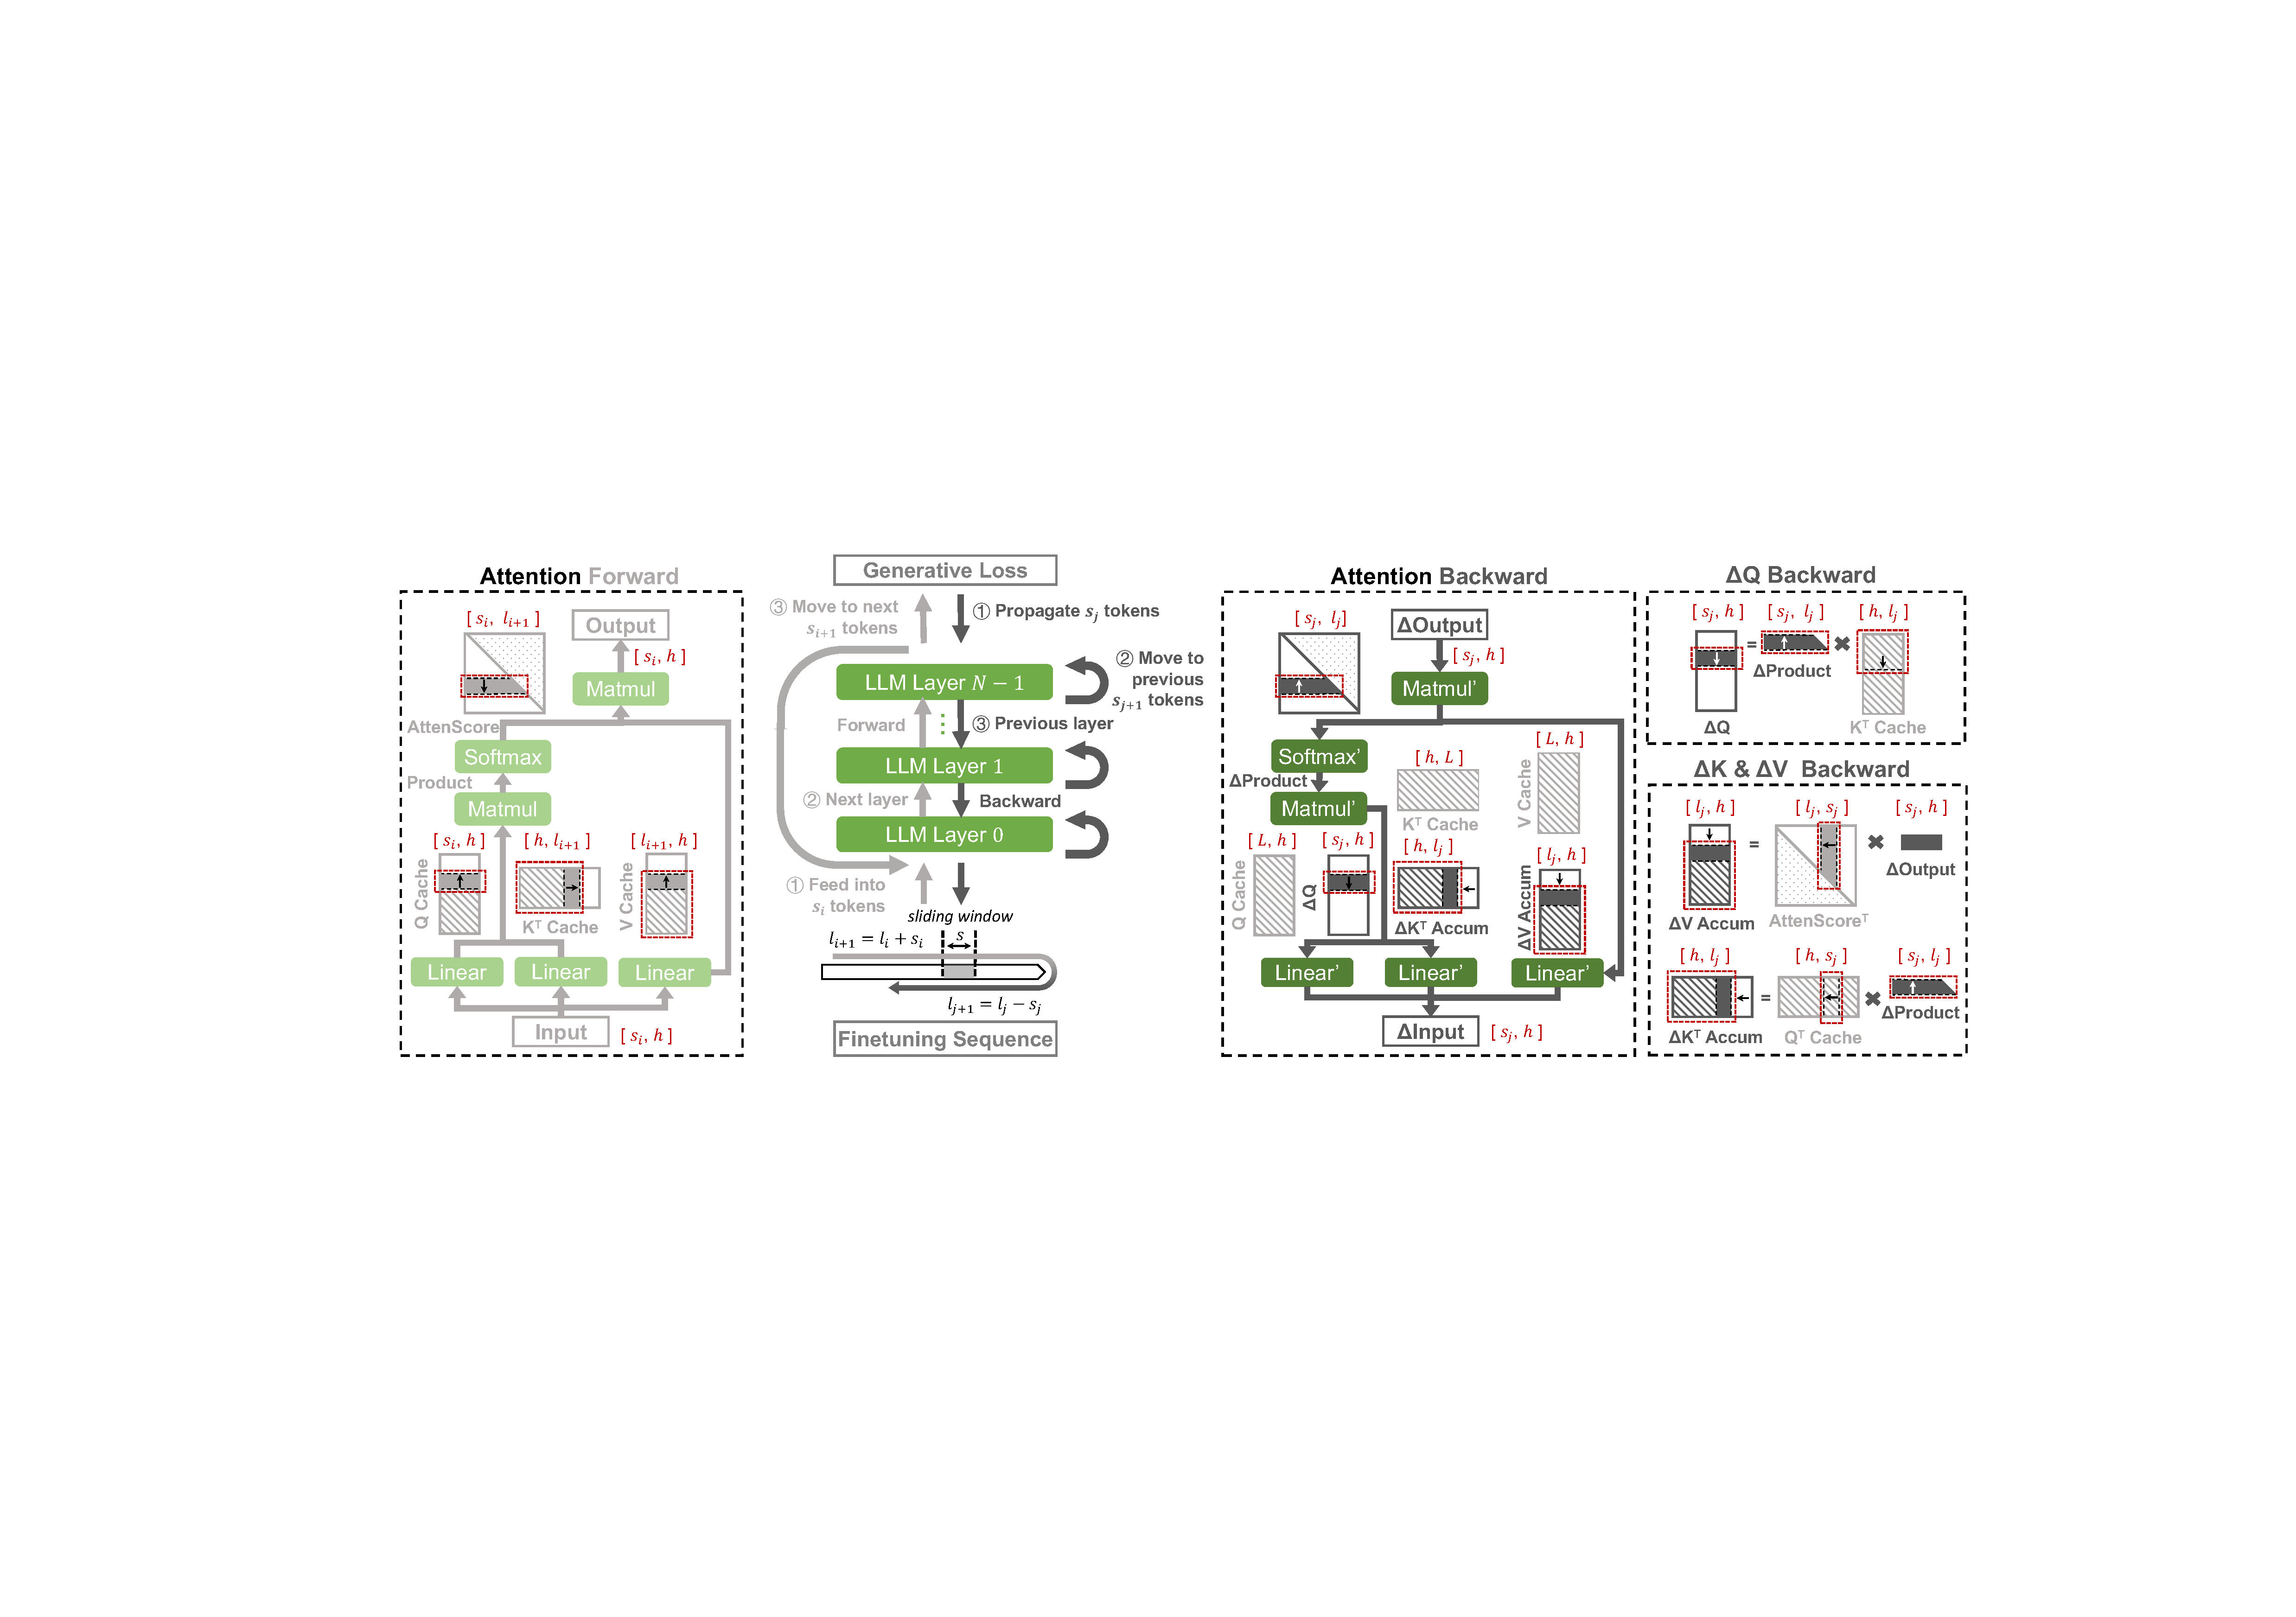
\includegraphics[width=\textwidth]{figs/tokenlevel2.pdf}
    \caption{Illustration of attention module's forward and backward execution with \sys's token-level finetuning mechanism.}
    \label{fig:token-level-finetuning}
\end{figure*}

\sys's {\em graph pruning} algorithm takes as input a PEFT model and its backbone LLM, and outputs a minimal set of intermediate activations that must be reserved to perform finetuning of the bypass networks.
%
This pruning process requires reasoning over data dependencies between operators, specifically their input and output tensors. Importantly, this pruning process preserves model quality since gradients with respect to frozen parameters are mathematically unnecessary for PEFT optimization and do not affect the final trained model. To facilitate the analysis of data dependencies, \sys introduces additional notation in the PCG representation.
Let $\m{G}=(\m{N}, \m{E})$ denote the PCG of a PEFT model, where each node $n \in \m{N}$ represents a tensor algebra (or parallelization) operator, and each edge $e=(n_1, n_2) \in \m{E}$ is a tensor shared between operators. For a node $n$, let $\m{I}(n)$ and $\m{O}(n)$ denote its set of input and output tensors.
%
By definition, $(n_1, n_2) \in \m{E}$ if and only if $\m{O}(n_1) \cap \m{I}(n_2) \neq \emptyset$, i.e., when at least one output tensor of $n_1$ serves as an input to $n_2$.
%

The design of \sys's graph pruning algorithm is based on two key observations.
%
First, conventional ML training procedures maintain all intermediate activations during the forward pass to compute gradients in the backward pass.
%
However, due to the linear algebra nature of most operators, these intermediate activations are primarily used to compute gradients with respect to the base LLM's trainable parameters. In the case of \peft, the backbone LLM parameters are frozen, and only the parameters in the bypass networks are updated.
%
This insight allows \sys to eliminate most intermediate activations, retaining only those necessary for computing gradients of the bypass networks. 
Second, different PEFT methods connect bypass networks at varying locations within the backbone LLMs, and therefore require different subsets of intermediate activations for backpropagation.
\Cref{fig:peft-methods} illustrates examples of how various \peft methods attach their bypass networks to the base LLM.

Building on these observations, \sys performs {\em static} graph pruning during the construction of the PCG for each registered \peft model, and {\em dynamical} scheduling to manage finetuning and inference tasks, along with corresponding memory allocations (see \Cref{sec:scheduling}).
%
\Cref{alg:graph_pruning} shows \sys's graph pruning algorithm, with \Cref{fig:graph_pruning} illustrating the process for an MLP model with LoRA. Given a PEFT model's PCG $\m{G}$, the algorithm generates an execution plan specifying which intermediate activations to cache for efficient backpropagation.

The algorithm constructs the backward graph $\overline{\m{G}}$ using reverse-mode automatic differentiation~\cite{hogan2014fast}, then prunes gradients for frozen base LLM weights. It iteratively processes operators to discover pruning opportunities, ultimately identifying the minimal set of activations $\m{A}$ required for the backward pass. \sys combines this with {\em rematerialization} and {\em activation compression}.
%

\paragraph{Rematerialization and compression.}
\sys applies tensor rematerialization~\cite{checkmate}, selectively discarding tensors in the forward pass and recomputing them during backpropagation. For each tensor $t \in \m{A}$ after graph pruning, \sys rematerializes $t$ if all input tensors are stored and recomputation has low overhead. Additionally, \sys opportunistically applies lossless compression when operators like {\tt ReLU} don't require access to original input tensors. 
$y=\texttt{ReLU}(x) = \max{(x, 0)}$ whose derivative is $\partial y/\partial x = 1$ for $x>0$ and $0$ for $x\leq0$. Therefore, instead of storing the original input tensor $x$, \sys keeps the bitmask of $x$.
